%%%%%%%%%%%%%%%%%%%%%%%%%%%%%%%%%%%%%%%%%%%%%%%%%%%%%%%%%%%%%%%%%%%%%%%%%%%%%%%
%
% Tommy P. Keane
% Master of Science Thesis
% Department of Electrical and Microelectronic Engineering
% Rochester Institute of Technology
%
% Presented: May 12, 2011
%
%%%%%%%%%%%%%%%%%%%%%%%%%%%%%%%%%%%%%%%%%%%%%%%%%%%%%%%%%%%%%%%%%%%%%%%%%%%%%%%
\documentclass{beamer}

\setbeamertemplate{caption}[numbered]

\usepackage{amsmath}
\usepackage{amssymb}
\usepackage{xfrac}
\usepackage{graphicx}
\graphicspath{{./images/}}
\usepackage{subfigure}

\usepackage{eulervm}

\bibliographystyle{unsrt}

\usetheme{Warsaw}


%%%%%%%%%%%%%%%%%%%%%%%%%%%%%%%%%%%%%%%%%%%%%%%%%%%%%%%%%%%%%%%%%%%%%%%%%%%%%%%
% FRONT MATTER
%%%%%%%%%%%%%%%%%%%%%%%%%%%%%%%%%%%%%%%%%%%%%%%%%%%%%%%%%%%%%%%%%%%%%%%%%%%%%%%
\title[M.S. Thesis: WFMI\hspace{10em}\insertframenumber{ }of \inserttotalframenumber]{\large\textsc{Weighted and Filtered Mutual Information}:
   \\
   A metric for automated creation of panoramas\\from views of complex scenes}
\author{Tommy P. Keane}
\institute{Thesis Defense Presentation \\ \vskip .1in Partial Fulfillment of the Degree of Master of Science \\ Department of Electrical and Microelectronic Engineering \\ Rochester Institute of Technology \\ Rochester, NY 14623 \\ \vskip .1in Presented on:}
\date{\vskip -.2in May 12, 2011}


%%%%%%%%%%%%%%%%%%%%%%%%%%%%%%%%%%%%%%%%%%%%%%%%%%%%%%%%%%%%%%%%%%%%%%%%%%%%%%%
% BEGIN DOCUMENT
%%%%%%%%%%%%%%%%%%%%%%%%%%%%%%%%%%%%%%%%%%%%%%%%%%%%%%%%%%%%%%%%%%%%%%%%%%%%%%%
\begin{document}

%%%%%%%%%%%%%%%%%%%%%%%%%%%%%%%%%%%%%%%%%%%%%%%%%%%%%%%%%%%%%%%%%%%%%%%%%%%%%%%
% TITLE SLIDE
\begin{frame}
\titlepage
\end{frame}



%%%%%%%%%%%%%%%%%%%%%%%%%%%%%%%%%%%%%%%%%%%%%%%%%%%%%%%%%%%%%%%%%%%%%%%%%%%%%%%
% ABSTRACT
%\begin{frame}[c]{Abstract}
%\noindent
%%%%%%%%%%%%%%%%%%%%%%%%%%%%%%%%%%%%%%%%%%%%%%%%%%%%%%%%%%%%%%%%%%%%%%%%%%%%%%%%%
%
% Tommy P. Keane
% Master of Science Thesis
% Department of Electrical and Microelectronic Engineering
%
% March 2011
%
%
%
%%%%%%%%%%%%%%%%%%%%%%%%%%%%%%%%%%%%%%%%%%%%%%%%%%%%%%%%%%%%%%%%%%%%%%%%%%%%%%%

%%%%%%%%%%%%%%%%%%%%%%%%%%%%%%%%%%%%%%%%%%%%%%%%%%%%%%%%%%%%%%%%%%%%%%%%%%%%%%%
%
% ABSTRACT
%
%%%%%%%%%%%%%%%%%%%%%%%%%%%%%%%%%%%%%%%%%%%%%%%%%%%%%%%%%%%%%%%%%%%%%%%%%%%%%%%


%%%%%%%%%%%%%%%%%%%%%%%%%%%%%%%%%%%%%%%%%%%%%%%%%%%%%%%%%%%%%%%%%%%%%%%%%%%%%%%
% BEGIN DOCUMENT
\begin{doublespace}

To contribute a novel approach in the field of image registration and panorama creation, this algorithm foregoes any scene knowledge, requiring only modest scene overlap and an acceptable amount of entropy within each overlapping view, both empirically derived. The weighted and filtered mutual information (WFMI) algorithm has been developed for stationary, color, surveillance video cameras and relies on color gradients for feature correspondence. This is a novel extension of well-established maximization of mutual information (MMI) algorithms. Where MMI algorithms are typically applied to high altitude photography and medical imaging (scenes with relatively simple shapes and affine homographies between views), the WFMI algorithm has been designed for scenes with occluded objects and significant parallax. Despite the typically non-affine surveillance scenarios, searching in the affine space is a practical assumption that provides computational efficiency and accurate results, even with complex scene views that suffer from parallax and occlusions. The WFMI algorithm can perfectly register affine views, performs exceptionally well with near-affine related views, and in complex (projective) views with parallax and occlusion the WFMI algorithm provides an accurate estimate of the overlap regions between the views. The WFMI algorithm uses simple calculations (vector field gradient, Laplacian filtering, and feature histograms) to generate the WFMI metric and provide the optimal affine relationship. This algorithm is unique when compared to typical MMI algorithms and modern registration algorithms because it avoids a lot of \textit{a priori} knowledge and calculations, while still providing an accurate or useful estimate for realistic scenes. With pixel based weightings and the Laplacian filtering operation, the WFMI algorithm overcomes the failures of typical MMI algorithms in scenes where complex or occluded shapes do not provide sufficiently large peaks in the mutual information maps. This work has currently been applied to individual video frames and future work could extend the algorithm into utilizing motion information or temporal frame registrations to enhance scenes with smaller overlap regions, lower entropy, or significant parallax and occlusions.

\end{doublespace}

%%%%%%%%%%%%%%%%%%%%%%%%%%%%%%%%%%%%%%%%%%%%%%%%%%%%%%%%%%%%%%%%%%%%%%%%%%%%%%%
% END OF DOCUMENT

%{\tiny This algorithm performs automatic registration by foregoing any scene knowledge, requiring only modest scene overlap and an acceptable amount of entropy within each overlapping view. The weighted and filtered mutual information (WFMI) algorithm has been developed for stationary, color, surveillance video cameras. This is a novel extension of maximization of mutual information (MMI) algorithms, which are typically applied to scenes with simple shapes and near-affine relationships between views. The WFMI algorithm has been designed for realistic, complex scenes with occlusion and parallax variations between the views. And despite the typically non-affine related surveillance scenarios, the WFMI algorithm is searching only in the affine space for computational efficiency. The WFMI algorithm can perfectly register affine views, performs exceptionally well with near-affine related views, and in complex (projective or polynomial related) views the WFMI algorithm provides an accurate estimate of the overlap region between the views. The WFMI algorithm uses simple calculations (vector field gradient, Laplacian filtering, and feature histograms) to generate the WFMI metric and provide the optimal affine relationship. This work has been applied to individual video frames and future work could extend the algorithm into utilizing motion information or temporal frame registrations to enhance the results.}
%\end{frame}

%\textsc{Reference}:
%\\
%{\tiny T. Keane, E. Saber, H. Rhody, A. Savakis, J. Raj, ''Unsupervised automated panorama creation for realistic surveillance scenes through weighted mutual information registration'', \textit{Proceedings of SPIE/IS\&T: Electronic Imaging Symposium}, San Francisco, CA, Jan. 2011}




%%%%%%%%%%%%%%%%%%%%%%%%%%%%%%%%%%%%%%%%%%%%%%%%%%%%%%%%%%%%%%%%%%%%%%%%%%%%%%%
% WHAT IS THE PROBLEM?
\begin{frame}[c]{\sc What is the Problem?}

\begin{center}

\begin{figure}[!h]
\centering
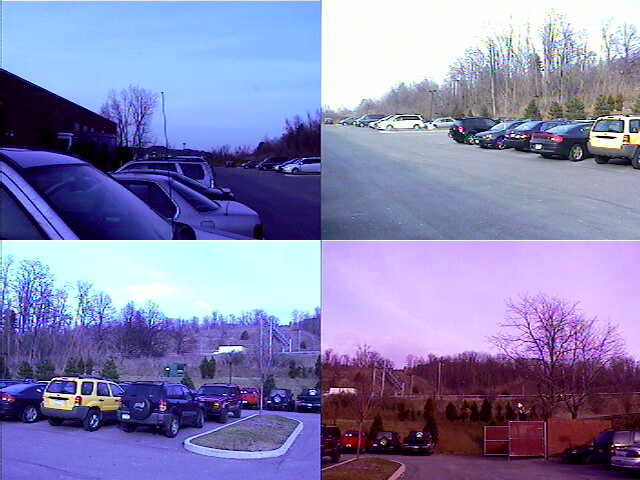
\includegraphics[width=.8\columnwidth]{LenelExample}
\caption{Lenel Parking Lot Example}
\label{LenelExample}
\end{figure}

\end{center}

\end{frame}



%%%%%%%%%%%%%%%%%%%%%%%%%%%%%%%%%%%%%%%%%%%%%%%%%%%%%%%%%%%%%%%%%%%%%%%%%%%%%%%
% WHAT IS AVAILABLE?
\begin{frame}[t]{\sc What is available?}

\begin{center}

\begin{figure}[!h]
\centering
\vfill
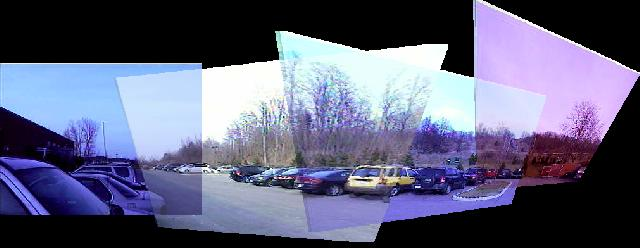
\includegraphics[width=1\columnwidth]{LenelExampleStitched}
\caption{Manually Registered Images from Figure \ref{LenelExample}}
\label{LenelExampleStitched}
\end{figure}

\end{center}

\end{frame}



%%%%%%%%%%%%%%%%%%%%%%%%%%%%%%%%%%%%%%%%%%%%%%%%%%%%%%%%%%%%%%%%%%%%%%%%%%%%%%%
% WHAT WAS OUR TASK?
\begin{frame}[c]{\sc What was our task?}

\begin{center}
{\sc Proposed}:
\\
Create an automated algorithm for registering, stitching, and blending the views from stationary color surveillance cameras.
\end{center}

\end{frame}


%%%%%%%%%%%%%%%%%%%%%%%%%%%%%%%%%%%%%%%%%%%%%%%%%%%%%%%%%%%%%%%%%%%%%%%%%%%%%%%
% WHAT HAS BEEN ACHIEVED?
\begin{frame}[t]{\sc What has been achieved?}

\vfill
\begin{center}
{\sc Weighted and Filtered Mutual Information (WFMI)}:
\\
A novel application of mutual information as a metric for determining overlapping portions of unconstrained views of complex, realistic scenes.
\\
\vskip .25in
Implementation in MATLAB\textsuperscript{\textregistered}, C++ with OpenCV
\\
\vskip .25in
Intellectual Property held by \\ Lenel Systems Inc., A UTC Fire and Security Corporation.
\end{center}

\end{frame}



%%%%%%%%%%%%%%%%%%%%%%%%%%%%%%%%%%%%%%%%%%%%%%%%%%%%%%%%%%%%%%%%%%%%%%%%%%%%%%%
% WHAT IS BEING PRESENTED?
\begin{frame}[t]{\sc What is being presented?}

\vfill

\begin{description}
\item[Multiple View Geometry] \hspace*{\fill} \\
System description and constraints.

\item[Mutual Information] \hspace*{\fill} \\
The how and why of the applied theory.

\item[Image Features] \hspace*{\fill} \\
What are they and how are they chosen?

\item[The Proposed Algorithm] \hspace*{\fill} \\
The design and implementation.

\item[Results and Constraints] \hspace*{\fill} \\
Synthetic and real-world examples and achievements.
\end{description}

\end{frame}




%%%%%%%%%%%%%%%%%%%%%%%%%%%%%%%%%%%%%%%%%%%%%%%%%%%%%%%%%%%%%%%%%%%%%%%%%%%%%%%
% IMAGE REGISTRATION 001
\begin{frame}[c]{\sc Image Registration}

\begin{figure}
\centering
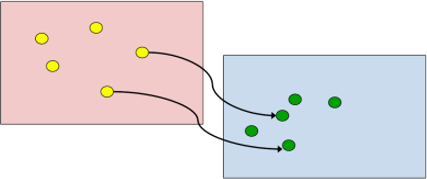
\includegraphics[width=.95\columnwidth]{imageRegistration}
\caption{Basic Idea of Image Registration}
\label{imageRegistration}
\end{figure}

\end{frame}



%%%%%%%%%%%%%%%%%%%%%%%%%%%%%%%%%%%%%%%%%%%%%%%%%%%%%%%%%%%%%%%%%%%%%%%%%%%%%%%
% IMAGE REGISTRATION 002
\begin{frame}[c]{\sc Finding Homographies}

\textbf{Affine Homography}:
\begin{equation}
\label{AffineHomographySolve}
\begin{bmatrix}\sfrac{\hat{x}}{1}\\\sfrac{\hat{y}}{1}\\1\end{bmatrix}=\begin{bmatrix}\hat{x}\\\hat{y}\\1\end{bmatrix}=\begin{bmatrix}a_{11}&a_{12}&a_{13}\\a_{21}&a_{22}&a_{23}\\0&0&1\end{bmatrix}\begin{bmatrix}x\\y\\1\end{bmatrix}
\end{equation}

\vfill

\textbf{Projective Homography}:
\begin{equation}
\label{ProjectiveHomographySolve}
\begin{bmatrix}\sfrac{\hat{x}}{\hat{z}}\\\sfrac{\hat{y}}{\hat{z}}\\1\end{bmatrix}=\begin{bmatrix}\hat{x}\\\hat{y}\\\hat{z}\end{bmatrix}=\begin{bmatrix}p_{11}&p_{12}&p_{13}\\p_{21}&p_{22}&p_{23}\\p_{31}&p_{32}&1\end{bmatrix}\begin{bmatrix}x\\y\\1\end{bmatrix}
\end{equation}

\end{frame}



%%%%%%%%%%%%%%%%%%%%%%%%%%%%%%%%%%%%%%%%%%%%%%%%%%%%%%%%%%%%%%%%%%%%%%%%%%%%%%%
% IMAGE REGISTRATION 003
\begin{frame}[t]{\sc Solving for Homographies}

\textbf{Direct Linear Transformation}:

\begin{center}

\vskip -0.15in
\begin{equation}
\label{DLT}
	A=\hat{\bf{x}}_{i} \times H \bf{x}_{i}=0
\end{equation}

\begin{equation}
\label{DLTSVD}
	A=U \Sigma V^{H}
\end{equation}

\begin{equation}
\label{SVD}
	\Sigma = \begin{bmatrix}\sigma_{1}&0&0&0&\cdots&0 \\ 0&\sigma_{2}&0&0&\cdots&0 \\ 0&0&\sigma_{3}&0&\cdots&0 \\ &&&\ddots&& \end{bmatrix}
\end{equation}

\end{center}

\end{frame}



%%%%%%%%%%%%%%%%%%%%%%%%%%%%%%%%%%%%%%%%%%%%%%%%%%%%%%%%%%%%%%%%%%%%%%%%%%%%%%%
% Describing Image Data
\begin{frame}[c]{\sc Describing Image Data}

\begin{figure}
\centering
\subfigure{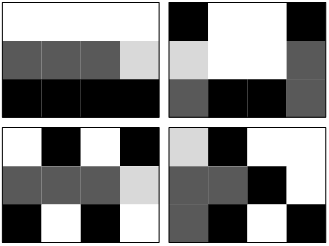
\includegraphics[width=.48\columnwidth]{sampleImages}}
\pause
\subfigure{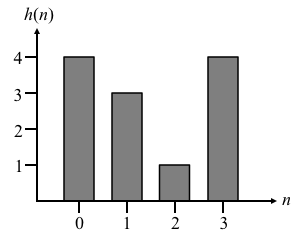
\includegraphics[width=.48\columnwidth]{sampleHistogram}}
\label{infoTheory2}
\end{figure}

\begin{block}<3->{Intensity Histogram}
Spatial data has been encoded, but cannot be uniquely decoded
\end{block}


\end{frame}


%%%%%%%%%%%%%%%%%%%%%%%%%%%%%%%%%%%%%%%%%%%%%%%%%%%%%%%%%%%%%%%%%%%%%%%%%%%%%%%
% DESCRIBING RANDOM VARIABLES
\begin{frame}[c]{\sc Describing Random Variables}


\begin{block}<1->{Probability Mass Function (PMF)}
The distribution of the random data in an image, found from the normalized histogram of the image data.
\begin{equation}
\label{PMF}
	p_{A}(\bf{a})=h_{A}(\bf{a}) \cdot \left(\sum_{i}{h_{A}(a_{i})} \right)^{-1} = \frac{h_{A}(\bf{a})}{\mathfrak{m}\cdot\mathfrak{n}}
\end{equation}
\end{block}

\vfill

\begin{block}<2->{Entropy}
The expected value of the self-information, thought of as the measure of randomness in the image data.
\begin{equation}
\label{entropy}
	H(A) = - \sum_{i}{p_{A}(a_{i}) \log_{n}{\left(p_{A}(a_{i})\right)}}
\end{equation}
\end{block}

\end{frame}



%%%%%%%%%%%%%%%%%%%%%%%%%%%%%%%%%%%%%%%%%%%%%%%%%%%%%%%%%%%%%%%%%%%%%%%%%%%%%%%
% WHY RANDOMNESS
\begin{frame}[c]{\sc Why Randomness?}

\only<1>
{\begin{figure}
\centering
\includegraphics[height=.8\textheight]{PinkBlock}
\label{infoTheory3}
\end{figure}
}

\only<2>
{\begin{figure}
\centering
\includegraphics[height=.8\textheight]{NoiseBlock}
\label{infoTheory3}
\end{figure}
}

\end{frame}



%%%%%%%%%%%%%%%%%%%%%%%%%%%%%%%%%%%%%%%%%%%%%%%%%%%%%%%%%%%%%%%%%%%%%%%%%%%%%%%
% DIAGRAM OF INFORMATION THEORY
\begin{frame}[c]{\sc Diagram of Information Theory}

\begin{figure}
\centering
\includegraphics[height=.7\textheight]{InformationTheoryVenn}
\caption{Venn diagram of key measures in Information Theory}
\label{infoTheory3}
\end{figure}

\end{frame}



% Understanding Information Theory
\begin{frame}[c]{\sc Understanding Information Theory}

\vskip -.25in
\begin{figure}
\centering
\subfigure{\includegraphics[width=.50\columnwidth]{InformationTheory3D_L}}
\subfigure{\includegraphics[width=.485\columnwidth]{InformationTheory3D_R}}
\label{infoTheory2}
\end{figure}

\vskip -.25in

\begin{equation}
H(A|B) = H(A,B) - H(B)
\end{equation}

\begin{equation}
H(B|A) = H(A,B) - H(A)
\end{equation}

\end{frame}




% Understanding Information Theory
\begin{frame}[c]{\sc Understanding Information Theory}

\vskip -.25in
\begin{figure}
\centering
\subfigure{\includegraphics[width=.48\columnwidth]{InformationTheory3D}}
\subfigure{\includegraphics[width=.48\columnwidth]{InformationTheoryVenn}}
\label{infoTheory2}
\end{figure}

\begin{equation}
I(A;B) = H(A) + H(B) - H(A,B)
\end{equation}

\end{frame}



%%%%%%%%%%%%%%%%%%%%%%%%%%%%%%%%%%%%%%%%%%%%%%%%%%%%%%%%%%%%%%%%%%%%%%%%%%%%%%%
% MUTUAL INFORMATION
\begin{frame}[c]{\sc Calculating Mutual Information}

\begin{block}<1->{Mutual Information}
The amount of knowledge that can be obtained about an image from knowledge about another image.

\begin{equation}
\label{MutualInformation}
	I(A;B) = \sum_{j}{\sum_{i}{p_{AB}(a_{i},b_{j}) \log_{2}{\left( \frac{p_{AB}(a_{i},b_{j})}{p_{A}(a_{i})p_{B}(b_{j})}\right)}}}
\end{equation}
%The difference between the expected value of the joint distribution self-information in the cases of dependence and independence.
\end{block}


\vfill

\begin{block}<2->{Normalized Mutual Information}
Symmetric Uncertainty.

\begin{equation}
\label{NormalizedMutualInformation}
	I_{N}(A;B) = \left( \frac{2}{H(A) + H(B)}\right) \cdot I(A;B)
\end{equation}
\end{block}

\end{frame}





%%%%%%%%%%%%%%%%%%%%%%%%%%%%%%%%%%%%%%%%%%%%%%%%%%%%%%%%%%%%%%%%%%%%%%%%%%%%%%%
% MOTION ESTIMATION

% MOTION ESTIMATION 001
\begin{frame}[c]{\sc Motion in Video}

\begin{figure}[!h]
\centering
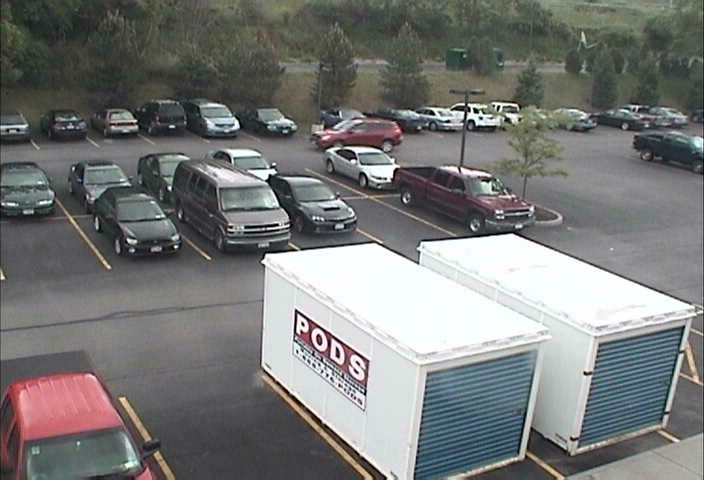
\includegraphics[width=.9\columnwidth]{Lenel010L(555)}
\caption{Lenel Parking Lot, Frame 555}
\label{Lenel555}
\end{figure}

\end{frame}

% MOTION ESTIMATION 001
\begin{frame}[c]{\sc Motion in Video}

\begin{figure}[!h]
\centering
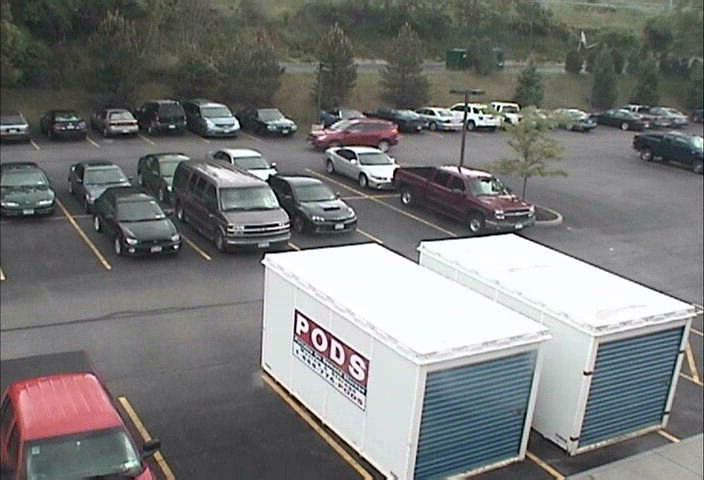
\includegraphics[width=.9\columnwidth]{Lenel010L(556)}
\caption{Lenel Parking Lot, Frame 556}
\label{Lenel556}
\end{figure}

\end{frame}

% MOTION ESTIMATION 001
\begin{frame}[c]{\sc Motion in Video}

\begin{figure}[!h]
\centering
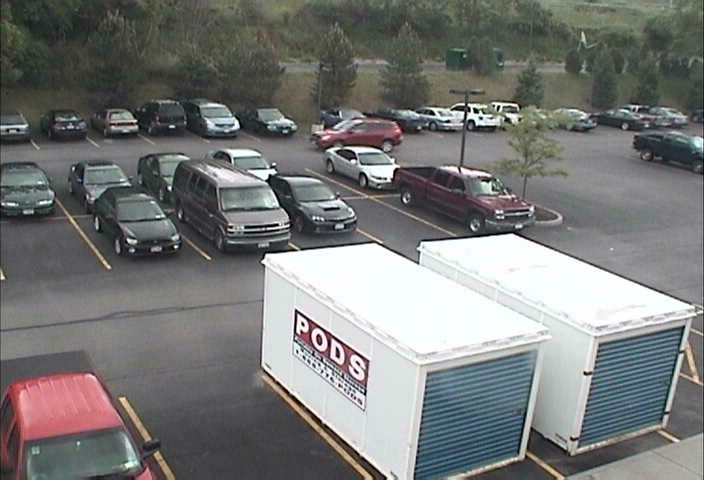
\includegraphics[width=.9\columnwidth]{Lenel010L(555)}
\caption{Lenel Parking Lot, Frame 555}
\label{Lenel555s}
\end{figure}

\end{frame}

% MOTION ESTIMATION 001
\begin{frame}[c]{\sc Motion in Video}

\begin{figure}[!h]
\centering
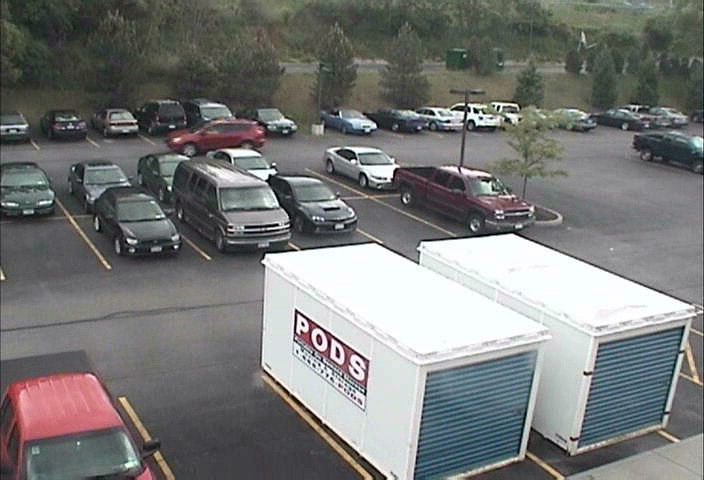
\includegraphics[width=.9\columnwidth]{Lenel010L(590)}
\caption{Lenel Parking Lot, Frame 590}
\label{Lenel590}
\end{figure}

\end{frame}


% MOTION ESTIMATION 002
\begin{frame}[c]{\sc Motion Estimation}

\begin{itemize}
\item Optical Flow Constraint
\item Gibbs Random Fields
\item Video Frame Registration
\item Gradient Descent Algorithms
\end{itemize}

\end{frame}





%%%%%%%%%%%%%%%%%%%%%%%%%%%%%%%%%%%%%%%%%%%%%%%%%%%%%%%%%%%%%%%%%%%%%%%%%%%%%%%
% DEPTH DETERMINATION

% DEPTH DETERMINATION 001
\begin{frame}[t]{\sc Depth Determination}

\begin{figure}[!h]
\centering
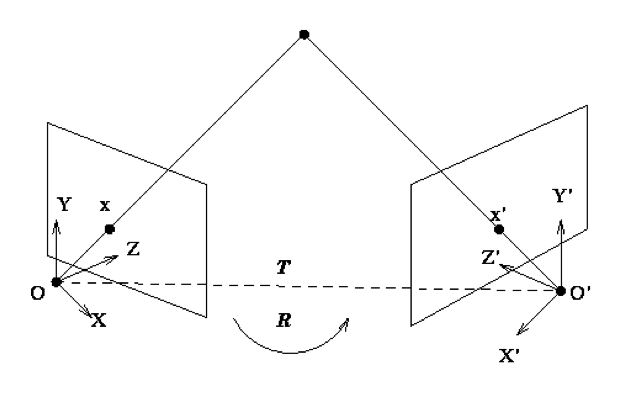
\includegraphics[width=.9\columnwidth]{CameraGeometry}
\caption{Multiple View Camera Geometry (Image from \cite{Hartley2003})}
\label{CameraGeometry}
\end{figure}

\end{frame}


%%%%%%%%%%%%%%%%%%%%%%%%%%%%%%%%%%%%%%%%%%%%%%%%%%%%%%%%%%%%%%%%%%%%%%%%%%%%%%%
% WFMI ALGORITHM

% ALGORITHM STEPS
\begin{frame}[c]{\sc WFMI Algorithm}
\begin{itemize}
\item Two Color Images
\item Color Gradient Maps
\item Histogram-Based Quantization of Color Gradients
\item Assume Image B as Reference, Transform Image A
\item Create Mutual Information Map through Translation Search
\item Weight the Mutual Information Map
\item Laplacian Filter the Weighted Mutual Information Map
\item Store Peak Value and Location
\item Move to next Transformation and Find next Peak
\item Take Maximum Peak and Transform Image A
\item Blend Images A and B
\end{itemize}
\end{frame}



\begin{frame}[c]{\sc WFMI Algorithm}

\begin{figure}[!h]
\centering
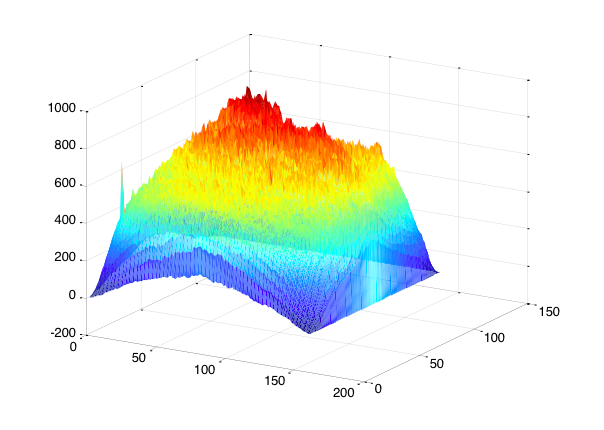
\includegraphics[height=.7\textheight]{MutualInformationMap}
\caption{Mutual Information Map from Translation Search}
\label{MutualInformationMap}
\end{figure}

\end{frame}


\begin{frame}[c]{\sc WFMI Algorithm}

\begin{figure}[!h]
\centering
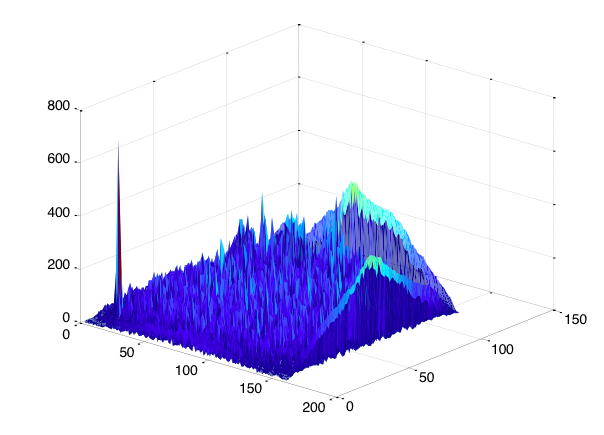
\includegraphics[height=.7\textheight]{FilteredMutualInformationMap}
\caption{Weighted and Filtered Mutual Information Map}
\label{FilteredMap}
\end{figure}

\end{frame}





\begin{frame}[c]{\sc WFMI Algorithm}

\begin{figure}[!h]
\centering
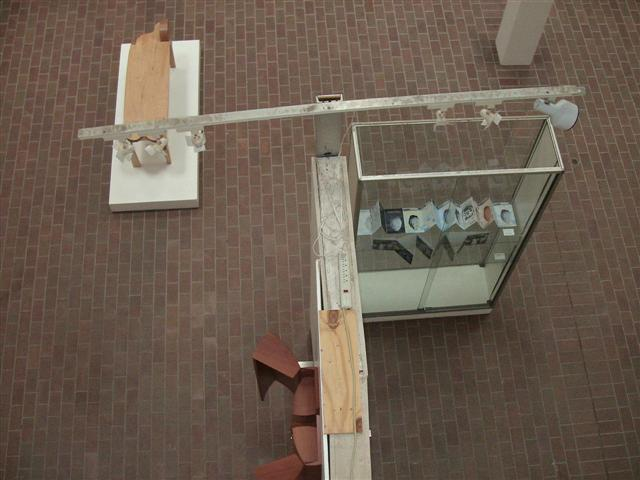
\includegraphics[height=.7\textheight]{AGS4L005}
\caption{Original Image}
\label{ArtGalleryOriginal}
\end{figure}

\end{frame}


\begin{frame}[c]{\sc WFMI Algorithm}

\begin{figure}[!h]
\centering
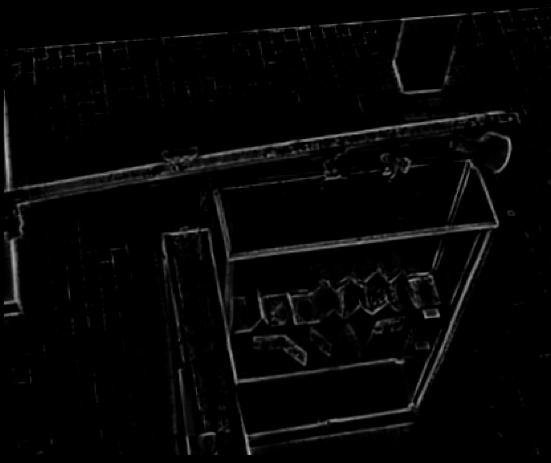
\includegraphics[height=.7\textheight]{ColorEdges}
\caption{Color Gradient Map \cite{Lee1991}}
\label{ArtGalleryGradient}
\end{figure}

\end{frame}


\begin{frame}[c]{\sc WFMI Algorithm}

\begin{figure}[!h]
\centering
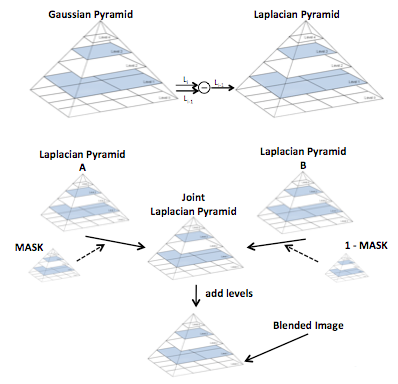
\includegraphics[height=.7\textheight]{MultiresolutionSpline}
\caption{Multiresolution Spline Blending \cite{Burt1983}}
\label{MultiresolutionSpline}
\end{figure}

\end{frame}







%%%%%%%%%%%%%%%%%%%%%%%%%%%%%%%%%%%%%%%%%%%%%%%%%%%%%%%%%%%%%%%%%%%%%%%%%%%%%%%
% WFMI RESULTS 001
\begin{frame}[c]{\sc Affine Frames}

\begin{figure}[!h]
\centering
\subfigure{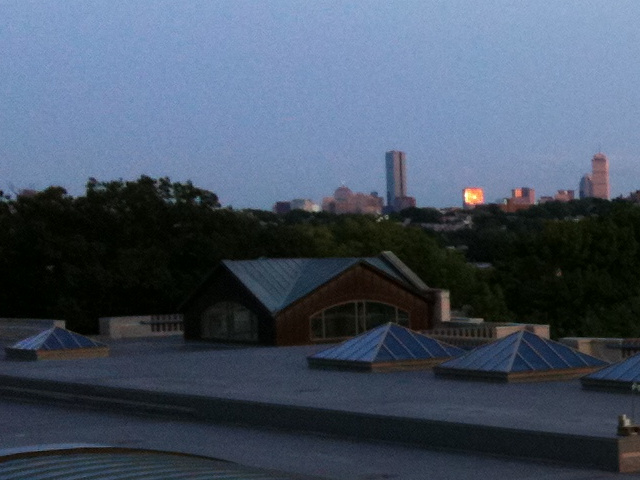
\includegraphics[width=.48\columnwidth]{RooftopL001} \label{RooftopL}}
\subfigure{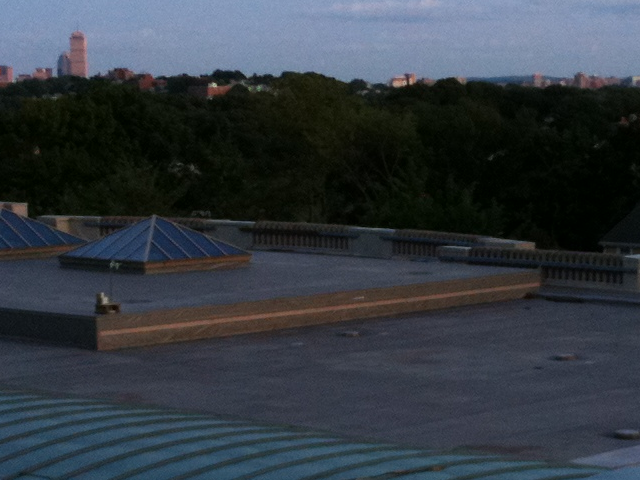
\includegraphics[width=.48\columnwidth]{RooftopR001} \label{RooftopR}}
\caption{Rooftop Scene (a) Left View, (b) Right View}
\label{RooftopImages}
\end{figure}

\end{frame}

% WFMI RESULTS 001
\begin{frame}[c]{\sc Affine Panorama}

\begin{figure}[!h]
\centering
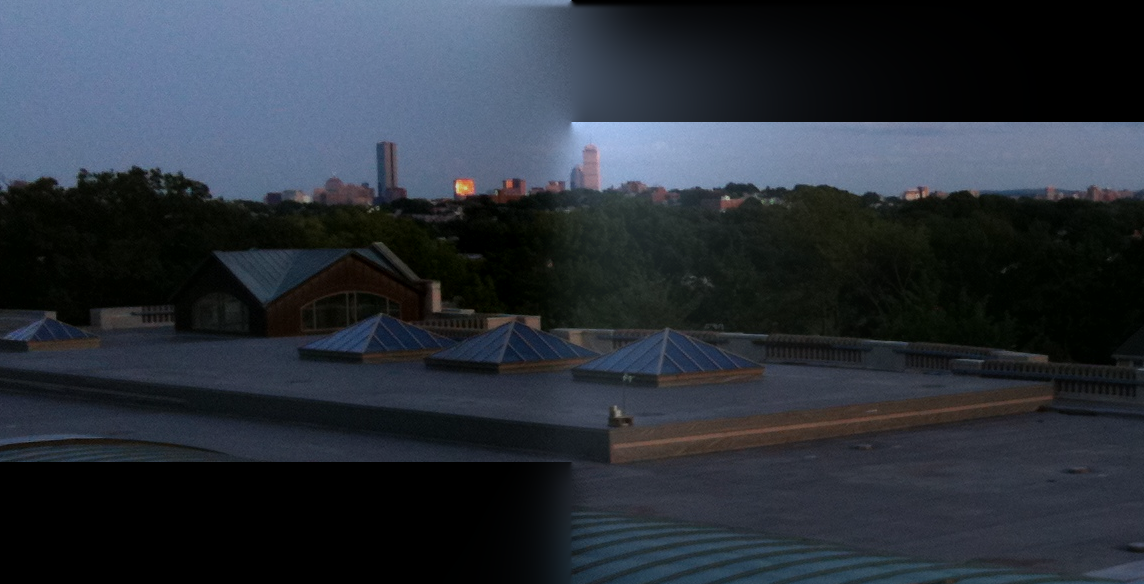
\includegraphics[width=1\columnwidth]{RooftopSP001001}
\caption{Rooftop Views Blended}
\label{RooftopStitched}
\end{figure}

\end{frame}


% WFMI RESULTS 002
\begin{frame}[c]{\sc Near Affine Frames}

\begin{figure}[!h]
\centering
\subfigure{ 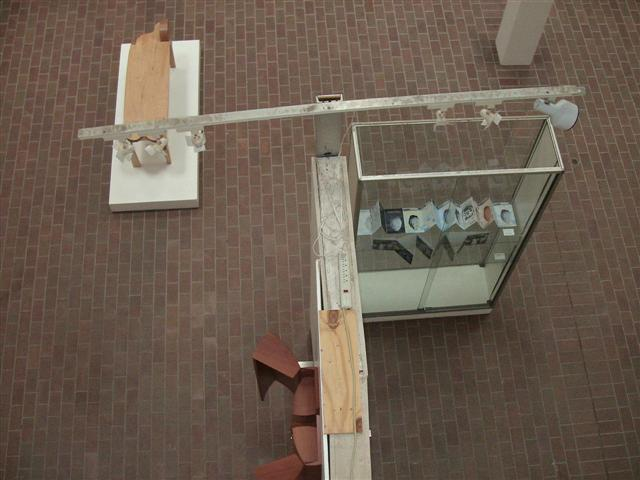
\includegraphics[width=.4\columnwidth]{AGS4L005} \label{ArtGallery4L} }
\subfigure{ 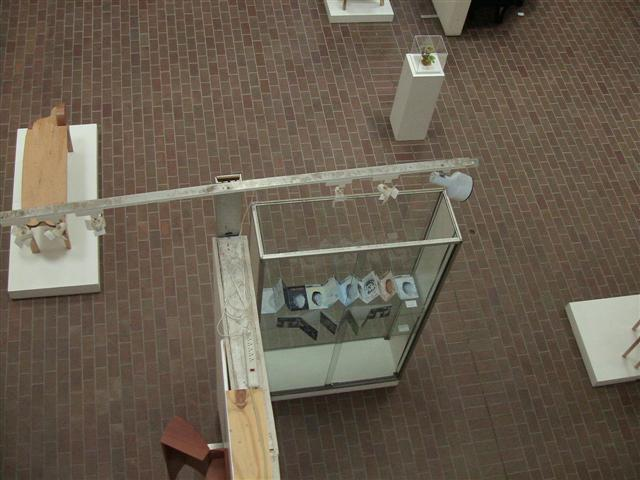
\includegraphics[width=.4\columnwidth]{AGS4R005} \label{ArtGallery4R} }
\caption{Art Gallery 04 Scene (a) Left View, (b) Right View}
\label{ArtGallery4Images}
\end{figure}

\end{frame}

% WFMI RESULTS 002
\begin{frame}[c]{\sc Near Affine Panorama}

\begin{figure}[!h]
\centering
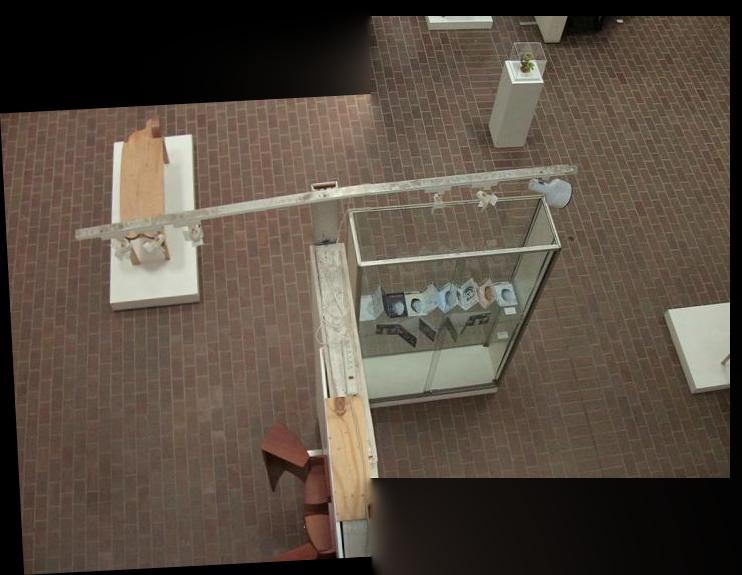
\includegraphics[width=.8\columnwidth]{AGS4SP005005}
\caption{Art Gallery 04 Views Blended}
\label{ArtGallery4Stitched}
\end{figure}

\end{frame}


% WFMI RESULTS 003
\begin{frame}[c]{\sc Complex Projective Frames}

\begin{figure}[!h]
\centering
\subfigure[]{ 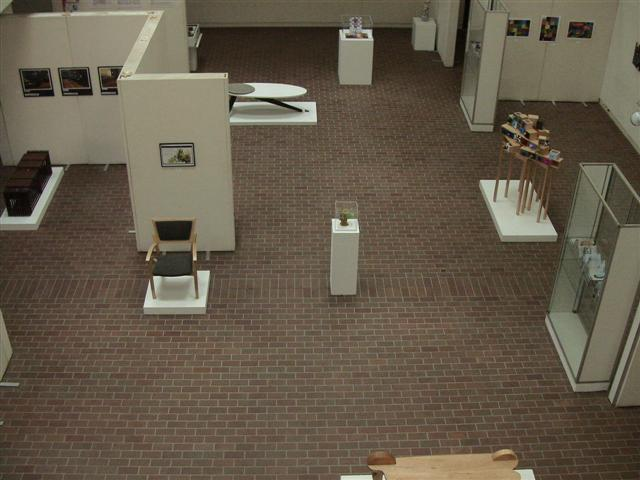
\includegraphics[width=.45\columnwidth]{AGS1L001} \label{ArtGallery1L} }
\subfigure[]{ 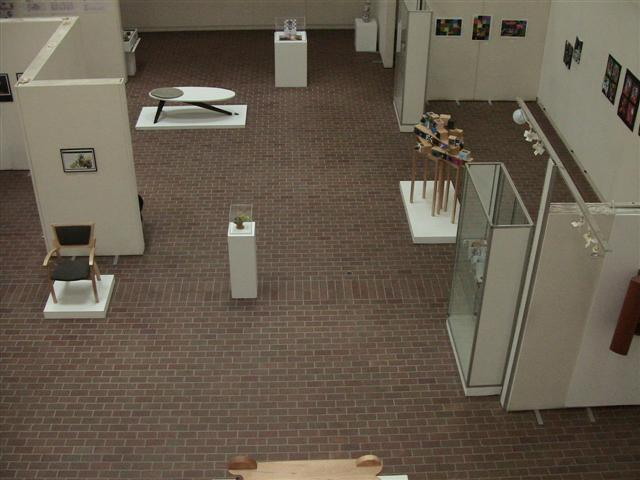
\includegraphics[width=.45\columnwidth]{AGS1R001} \label{ArtGallery1R} }
\caption{Art Gallery Scene 01 (a) Left View, (b) Right View}
\label{ArtGallery1Images}
\end{figure}

\end{frame}

% WFMI RESULTS 003
\begin{frame}[c]{\sc Complex Projective Panorama}

\begin{figure}[!h]
\centering
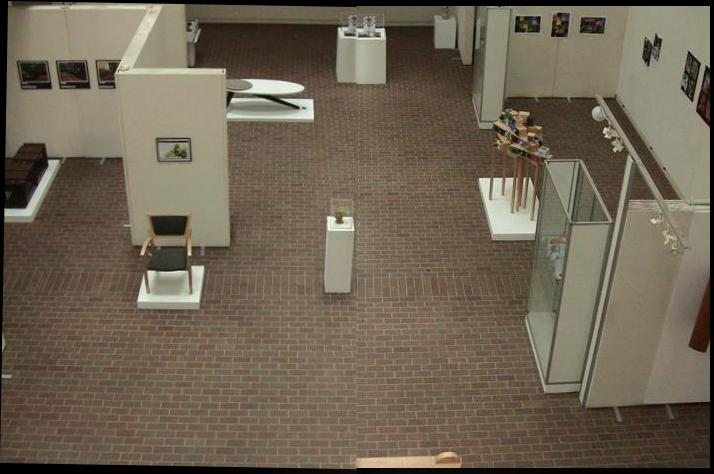
\includegraphics[width=.9\columnwidth]{AGS1SP001001}
\caption{Art Gallery 01 Views Blended}
\label{ArtGallery1Stitched}
\end{figure}

\end{frame}


% WFMI RESULTS 004
\begin{frame}[c]{\sc Complex Projective Frames}

\begin{figure}[!h]
\centering
\subfigure[]{ 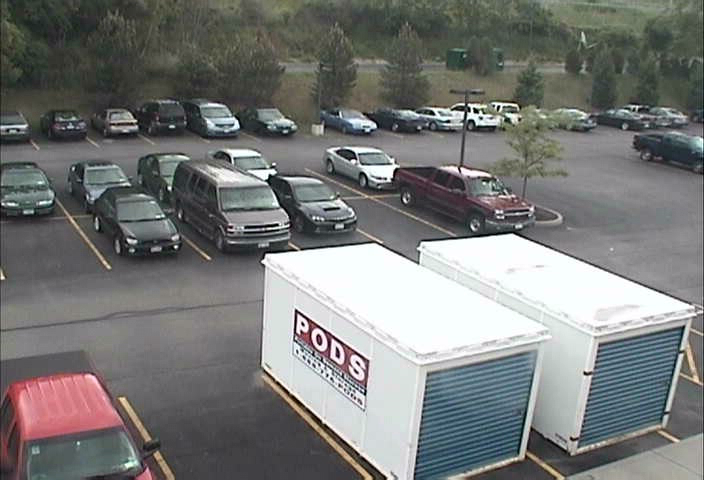
\includegraphics[width=.45\columnwidth]{Lenel010L004} \label{Lenel10L} }
\subfigure[]{ 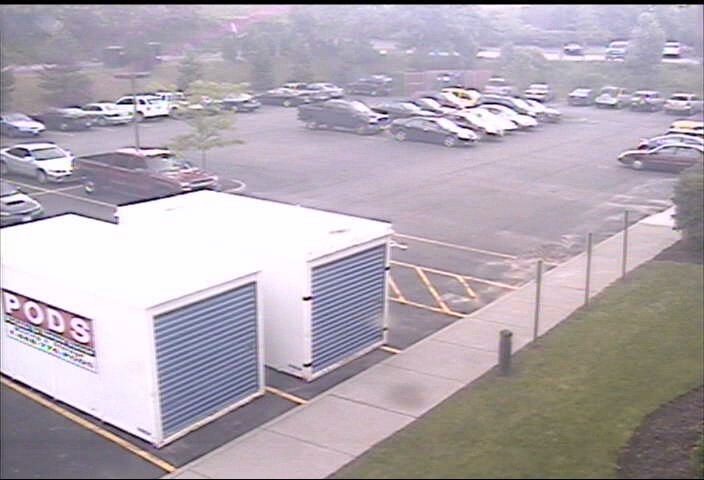
\includegraphics[width=.45\columnwidth]{Lenel010R004} \label{Lenel10R} }
\caption{Lenel Back Lot Scene (a) Left View, (b) Right View}
\label{Lenel10Images}
\end{figure}

\end{frame}

% WFMI RESULTS 004
\begin{frame}[c]{\sc Complex Projective Panorama}

\begin{figure}[!h]
\centering
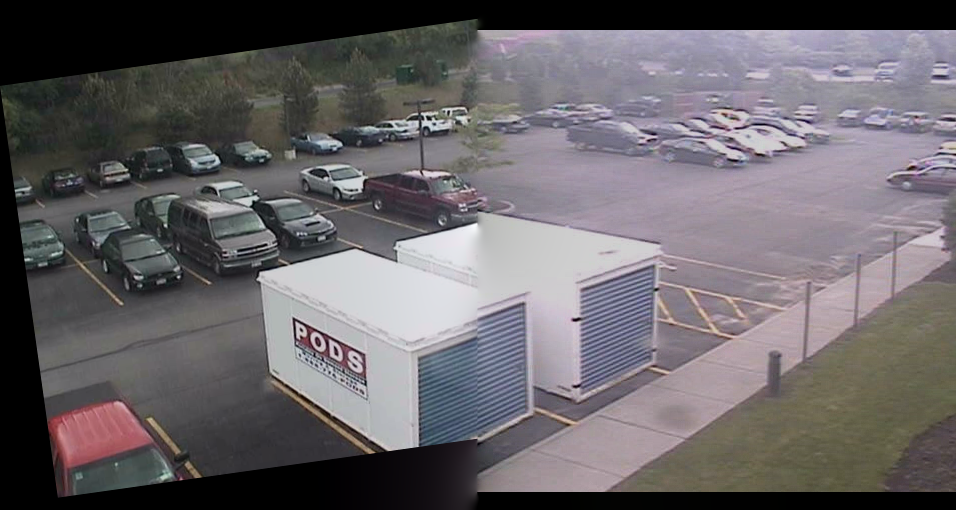
\includegraphics[width=1\columnwidth]{Lenel010SP001}
\caption{Lenel Back Lot Views Blended}
\label{Lenel10Stitched}
\end{figure}

\end{frame}



%%%%%%%%%%%%%%%%%%%%%%%%%%%%%%%%%%%%%%%%%%%%%%%%%%%%%%%%%%%%%%%%%%%%%%%%%%%%%%%
% CONCLUSION
\begin{frame}[c]{\sc Conclusion}
\begin{itemize}
\item Novel Application of Mutual Information
\item Realistic Scenes and Practical Concerns
\item Concepts Theoretically Extensible to Motion Estimation
\item Concepts Theoretically Extensible to Depth Determination
\item Not well-worn Research Territory
\end{itemize}
\end{frame}


%%%%%%%%%%%%%%%%%%%%%%%%%%%%%%%%%%%%%%%%%%%%%%%%%%%%%%%%%%%%%%%%%%%%%%%%%%%%%%%
% DEDICATION

\begin{frame}[c]{Dedication}
%%%%%%%%%%%%%%%%%%%%%%%%%%%%%%%%%%%%%%%%%%%%%%%%%%%%%%%%%%%%%%%%%%%%%%%%%%%%%%%%
%
% Tommy P. Keane
% Master of Science Thesis
% Department of Electrical and Microelectronic Engineering
%
% March 2011
%
%
%
%%%%%%%%%%%%%%%%%%%%%%%%%%%%%%%%%%%%%%%%%%%%%%%%%%%%%%%%%%%%%%%%%%%%%%%%%%%%%%%

%%%%%%%%%%%%%%%%%%%%%%%%%%%%%%%%%%%%%%%%%%%%%%%%%%%%%%%%%%%%%%%%%%%%%%%%%%%%%%%
%
% DEDICATION
%
%%%%%%%%%%%%%%%%%%%%%%%%%%%%%%%%%%%%%%%%%%%%%%%%%%%%%%%%%%%%%%%%%%%%%%%%%%%%%%%


%%%%%%%%%%%%%%%%%%%%%%%%%%%%%%%%%%%%%%%%%%%%%%%%%%%%%%%%%%%%%%%%%%%%%%%%%%%%%%%
% BEGIN DOCUMENT
\begin{center}

\vfill

\textit{[REDACTED; 2023]}

\end{center}

\vfill

%%%%%%%%%%%%%%%%%%%%%%%%%%%%%%%%%%%%%%%%%%%%%%%%%%%%%%%%%%%%%%%%%%%%%%%%%%%%%%%
% END OF DOCUMENT

\centering
[REDACTED; 2023]

\end{frame}



%%%%%%%%%%%%%%%%%%%%%%%%%%%%%%%%%%%%%%%%%%%%%%%%%%%%%%%%%%%%%%%%%%%%%%%%%%%%%%%
% ACKNOWLEDGEMENTS
\begin{frame}[c]{Acknowledgments}
%%%%%%%%%%%%%%%%%%%%%%%%%%%%%%%%%%%%%%%%%%%%%%%%%%%%%%%%%%%%%%%%%%%%%%%%%%%%%%%%
%
% Tommy P. Keane
% Master of Science Thesis
% Department of Electrical and Microelectronic Engineering
%
% March 2011
%
%
%
%%%%%%%%%%%%%%%%%%%%%%%%%%%%%%%%%%%%%%%%%%%%%%%%%%%%%%%%%%%%%%%%%%%%%%%%%%%%%%%

%%%%%%%%%%%%%%%%%%%%%%%%%%%%%%%%%%%%%%%%%%%%%%%%%%%%%%%%%%%%%%%%%%%%%%%%%%%%%%%
%
% ACKNOWLEDGMENTS
%
%%%%%%%%%%%%%%%%%%%%%%%%%%%%%%%%%%%%%%%%%%%%%%%%%%%%%%%%%%%%%%%%%%%%%%%%%%%%%%%


%%%%%%%%%%%%%%%%%%%%%%%%%%%%%%%%%%%%%%%%%%%%%%%%%%%%%%%%%%%%%%%%%%%%%%%%%%%%%%%
% BEGIN DOCUMENT

\begin{doublespace}

\textit{[REDACTED; 2023]}

\vfill
\end{doublespace}


%%%%%%%%%%%%%%%%%%%%%%%%%%%%%%%%%%%%%%%%%%%%%%%%%%%%%%%%%%%%%%%%%%%%%%%%%%%%%%%
% END OF DOCUMENT

\centering
[REDACTED; 2023]

\end{frame}


%%%%%%%%%%%%%%%%%%%%%%%%%%%%%%%%%%%%%%%%%%%%%%%%%%%%%%%%%%%%%%%%%%%%%%%%%%%%%%%
% REFERENCES
\begin{frame}[allowframebreaks]{\sc References}
\tiny
\bibliography{../LaTeX_Thesis/TommyKeane_MS_Thesis_Bibliography}
\nocite{*}
\end{frame}

%%%%%%%%%%%%%%%%%%%%%%%%%%%%%%%%%%%%%%%%%%%%%%%%%%%%%%%%%%%%%%%%%%%%%%%%%%%%%%%
% END OF DOCUMENT
%%%%%%%%%%%%%%%%%%%%%%%%%%%%%%%%%%%%%%%%%%%%%%%%%%%%%%%%%%%%%%%%%%%%%%%%%%%%%%%
\end{document}
